Let
\begin{align}
\vec{A} = \myvec
{
-1 \\
 2\\
},
\vec{C} = 
\myvec
{
3\\
2\\
}
\end{align}
The given square is available in \figref{fig:7/4/4/4Fig1}.
\figref{fig:7/4/4/4Fig2} shows the translation of $\vec{A}$ to the origin. 
\figref{fig:7/4/4/4Fig3} shows the subsequent anticlockwise rotation of the square by $45\degree$.
From
	\eqref{eq:conic_affine}.
\begin{align}
\vec{C} - \vec{A} = \myvec{
4\\
0
} \equiv 
\myvec{
1\\
0
},\,
\phi= 0\degree
\end{align}
		where
$\phi$ is the angle made by $AC$ with the x-axis.
Substituting numerical values in 
	\eqref{eq:affine-square-bd},
\begin{align}
	\vec{B}
	=2\myvec{1 & 1 \\ -1 & 1}\myvec{1\\0}+
\myvec
{
-1 \\
 2\\
}
=
\myvec{
1\\
0
}.
		\end{align}
		Similarly,
\begin{align}
\vec{D} = 
\myvec{
1\\
4
}.
\end{align}
\begin{figure}[!ht]
	\begin{center} 
	    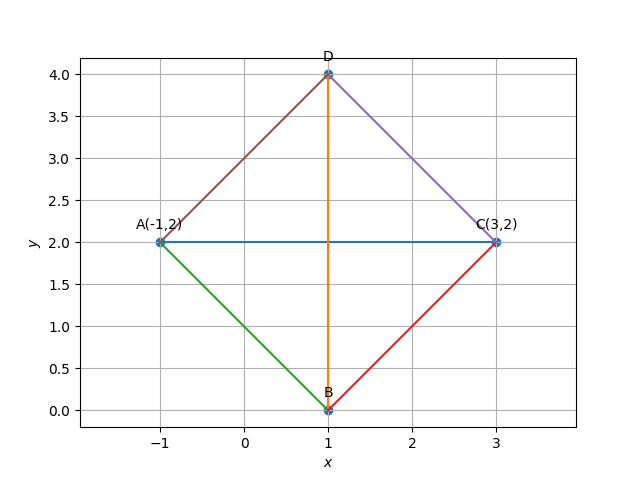
\includegraphics[width=\columnwidth]{chapters/10/7/4/4/figs/square}
	\end{center}
\caption{}
\label{fig:7/4/4/4Fig1}
\end{figure}
\begin{figure}[!h]
	\begin{center} 
	    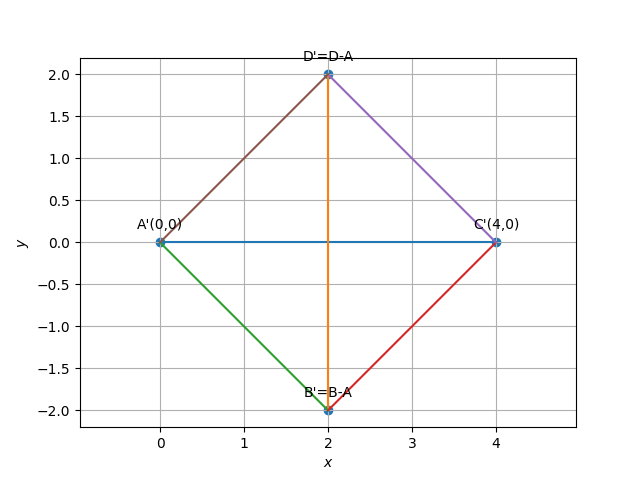
\includegraphics[width=\columnwidth]{chapters/10/7/4/4/figs/square1}
	\end{center}
\caption{}
\label{fig:7/4/4/4Fig2}
\end{figure}
\begin{figure}[!h]
	\begin{center} 
	    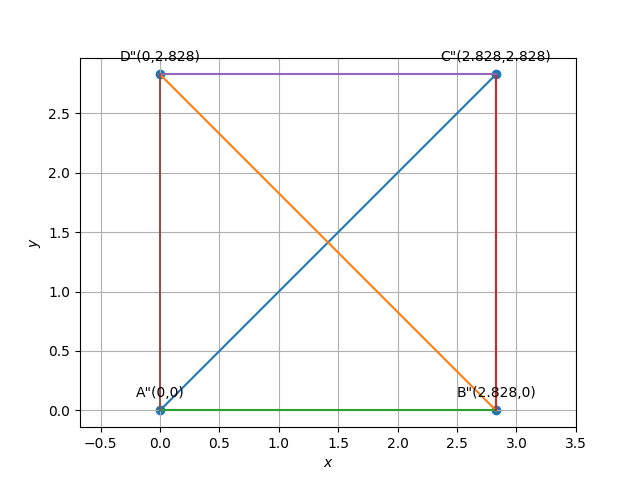
\includegraphics[width=\columnwidth]{chapters/10/7/4/4/figs/square2}
	\end{center}
\caption{}
\label{fig:7/4/4/4Fig3}
\end{figure}
